\section{Regiomontanus and the Birth of Trigonometry as a Discipline}

\subsection{From Tables to Theory: Regiomontanus Defines Trigonometry}

By the 15th century, European mathematics was beginning to reawaken — and one of its clearest signs was the appearance of a book that, for the first time, treated trigonometry as an independent mathematical subject.

That book was \textit{De Triangulis Omnimodis} (On Triangles of Every Kind), written around 1464 by the German mathematician \textbf{Johann Müller}, better known as \textbf{Regiomontanus}.

Unlike earlier astronomers who embedded trigonometry within celestial models or tables, Regiomontanus organized it as a coherent mathematical system. His work drew heavily from Islamic sources — particularly the chord-based trigonometry of Al-Battani and Al-Tusi — but restructured them using the evolving notational tools of Renaissance Europe.

\textbf{What made \textit{On Triangles} groundbreaking?}

\begin{itemize}
  \item It was the first European text to treat \textbf{trigonometry as a branch of mathematics} — not just a tool for astronomy.
  \item It gave explicit attention to both \textbf{plane} and \textbf{spherical triangles}, covering the general rules for solving them.
  \item It included clear statements of what we now call the \textbf{Law of Sines} and \textbf{Law of Cosines}.
  \item It synthesized Greek geometry and Islamic trigonometric techniques using Latin terminology and notation.
\end{itemize}

Regiomontanus was also a practicing astronomer and instrument-maker, and his goal was practical as well as theoretical: to provide accurate methods for celestial navigation, eclipse prediction, and positional astronomy — all through a unified geometric lens.


\subsection{Regiomontanus’ Trigonometry: Measuring the Firmament with Triangles}

For Regiomontanus, trigonometry wasn’t just abstract mathematics — it was a way to map the heavens.

In \textit{De Triangulis Omnimodis}, he systematically organized the rules for solving both \textbf{plane} and \textbf{spherical triangles}. While today these distinctions are part of standard curricula, in the 15\textsuperscript{th} century, this was revolutionary — especially because spherical trigonometry was the key to unlocking the geometry of the cosmos.

Regiomontanus built his system around fundamental relationships we now recognize as:

\begin{itemize}
  \item The \textbf{Law of Sines}:
  \[
  \frac{\sin A}{a} = \frac{\sin B}{b} = \frac{\sin C}{c}
  \]
  for plane triangles, and its spherical counterpart adapted for arcs on a sphere.
  
  \item The \textbf{Law of Cosines} for both plane and spherical triangles, allowing computation of unknown sides or angles when direct measurement was impossible.
\end{itemize}

He replaced the older chord-based methods inherited from Ptolemy and Islamic astronomers with a more streamlined sine-based approach, which made calculations simpler and more versatile.

But this wasn’t math for math’s sake. Regiomontanus had his eyes on the sky.



\begin{figure}[H]
  \centering
  \begin{tikzpicture}[scale=1.2, every node/.style={font=\small}]
    % === Plane triangle ===
    \begin{scope}[shift={(-4,0)}]
      % vertices
      \coordinate (A) at (0,0);
      \coordinate (B) at (3,0);
      \coordinate (C) at (1.2,2);
      % sides with labels
      \draw (A) -- node[midway, below] {$c$} (B)
            (B) -- node[midway, right] {$a$} (C)
            (C) -- node[midway, left]  {$b$} (A);
      % angle‐labels
      \node[below left]  at (A) {$A$};
      \node[below right] at (B) {$B$};
      \node[above]       at (C) {$C$};
      % optional little arcs to mark angles
      \draw pic["$\alpha$", draw=black, angle radius=6mm] {angle=C--A--B};
      \draw pic["$\beta$",  draw=black, angle radius=6mm] {angle=A--B--C};
      \draw pic["$\gamma$", draw=black, angle radius=6mm] {angle=B--C--A};
      \node at (1.5,-1) {Plane triangle};
    \end{scope}

    % === Spherical triangle ===
    \begin{scope}[shift={(4,0)}]
      % circle for sphere’s great circle
      \draw (0,0) circle (2cm);
      % three points on the “sphere”
      \coordinate (A') at (110:2cm);
      \coordinate (B') at (10:2cm);
      \coordinate (C') at (250:2cm);
      \node[fill=black, circle, inner sep=1.2pt] at (A') {};
      \node[fill=black, circle, inner sep=1.2pt] at (B') {};
      \node[fill=black, circle, inner sep=1.2pt] at (C') {};
      % great-circle arcs as triangle edges
      \draw[thick] (A') arc[start angle=110,end angle=10,radius=2cm]
                   node[midway, above right] {$c$};
      \draw[thick] (B') arc[start angle=10,end angle=250,radius=2cm]
                   node[midway, below right] {$a$};
      \draw[thick] (C') arc[start angle=250,end angle=110,radius=2cm]
                   node[midway, left] {$b$};
      % vertex labels
      \node[above left]  at (A') {$A$};
      \node[above right] at (B') {$B$};
      \node[below]       at (C') {$C$};
      \node at (0,-2.5) {Spherical triangle};
    \end{scope}
  \end{tikzpicture}
  \caption{Left: a plane triangle with sides \(a,b,c\) opposite angles \(A,B,C\) (Law of Sines). Right: a spherical triangle on great‐circle arcs of lengths \(a,b,c\) between vertices \(A,B,C\).}
\end{figure}


\begin{figure}[H]
  \centering
  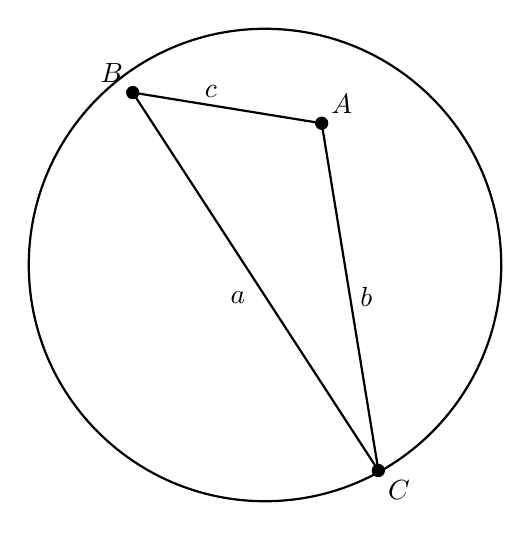
\begin{tikzpicture}[scale=3, x={(0.8cm,-0.4cm)}, y={(0cm,0.9cm)}]
    % A very rough oblique projection of a circle (the “sphere”)
    \draw[thick] (0,0) circle (1cm);
    % Three projected points on that “sphere”
    \coordinate (A) at (  0.3,  0.8);
    \coordinate (B) at (-0.7,  0.5);
    \coordinate (C) at (  0.6, -0.7);
    % straight‐line segments approximate the great‐circle arcs
    \draw[thick] (A) -- (B) node[midway, above left]  {$c$};
    \draw[thick] (B) -- (C) node[midway, below left]  {$a$};
    \draw[thick] (C) -- (A) node[midway, right]      {$b$};
    % vertices
    \fill (A) circle (0.8pt) node[above right] {$A$};
    \fill (B) circle (0.8pt) node[above left]  {$B$};
    \fill (C) circle (0.8pt) node[below right] {$C$};
  \end{tikzpicture}
  \caption{Oblique-projection “3D” view of a spherical triangle.}
\end{figure}



\begin{figure}[H]
  \centering
  \begin{mplibcode}
    input featpost;

    beginfig(3);
      numeric u, basesize, baseheight, alphang, thetang, sfearsize;
      numeric armsize, marginraise, totalraise, axeray, cardansize;
      color basepos, tdorigin, oneaxe, otheraxe, rotaxbascenter, axedir;
      color gluaxbascenter, rotrajcenter, cardanpos, refpoint, anotheraxe;
      color armdir, armbasonepos, armbastwopos, sfearpos;
      path glueaxebase, rotataxebase, rotrajector, axepath, sfearpath;
      numeric armray;
      u = 0.0125mm;
      basesize = 30u;
      baseheight = 3u;
      alphang = 20;
      thetang = -18;
      armsize = 25u;
      marginraise = 6u;
      axeray = 3u;
      cardansize = 3u;
      sfearsize = 4u;
      armray = 1.5u;
      totalraise = armsize*sind(alphang)+marginraise+cardansize*cosd(alphang);
      basepos = (0,0,-0.5baseheight);
      f := -2*(-2basesize,-basesize,-5baseheight);
      kindofcube(false, false, basepos, 0, 0, 0, 2basesize, 2basesize, baseheight );
      tdorigin = (0,0,0);
      oneaxe = (0,axeray/cosd(alphang),0);
      otheraxe = (1,0,0);
      anotheraxe = (0,cosd(alphang),-sind(alphang));
      gluaxbascenter = tdorigin - (0,totalraise*sind(alphang),0);
      glueaxebase = ellipticpath( gluaxbascenter, oneaxe, axeray*otheraxe );
      axedir = (0,sind(alphang),cosd(alphang));
      rotrajcenter = (0,0,totalraise);
      rotaxbascenter = rotrajcenter-axedir*cardansize;
      refpoint = rotrajcenter+axedir*cardansize;
      rotataxebase = rigorouscircle( rotaxbascenter, axedir, axeray );
      rotrajector = rigorouscircle( rotrajcenter, axedir, armsize );
      axepath = twocyclestogether( glueaxebase, rotataxebase );
      fill axepath withcolor background;
      draw axepath;
      draw rotataxebase;
      drawarrow subpath (3,10.5) of rotrajector dashed evenly;
    %  dotlabel.top( btex 1 etex, point 1 of rotrajector );
    %  dotlabel.top( btex 5 etex, point 5 of rotrajector );
    %  dotlabel.top( btex 3 etex, point 3 of rotrajector );
      kindofcube(false,false,rotrajcenter,90,90-alphang,thetang,2cardansize,2cardansize,2cardansize);
      draw rp(refpoint);
      armdir := otheraxe*cosd(thetang)+anotheraxe*sind(thetang);
      armbasonepos = rotrajcenter + cardansize*armdir;
      armbastwopos = rotrajcenter + (armsize-sfearsize)*armdir; % NOT RIGOROUS
      sfearpos = rotrajcenter + armsize*armdir;
      rigorousdisc( 0, true, armbasonepos, armray, armbastwopos-armbasonepos );
      sfearpath = rigorousfearpath( sfearpos, sfearsize );
      fill sfearpath withcolor background;
      draw sfearpath;
  endfig;
  
  \end{mplibcode}
  \caption{A 3D perspective‐projected spherical triangle rendered via MetaPost in mplibcode.}
\end{figure}








\subsection{Applying Trigonometry to the Firmament}

Like his predecessors, Regiomontanus operated within a geocentric cosmology. The firmament — the outermost celestial sphere containing the fixed stars — was still considered a real, rotating structure. To predict planetary positions, chart eclipses, or navigate by the stars, one had to compute angles and distances on this imagined sphere.

Spherical trigonometry was the language of the heavens.

Regiomontanus applied his methods to:

\begin{itemize}
  \item Calculate the apparent positions of celestial bodies on the rotating celestial sphere.
  \item Determine angular separations between stars — critical for astronomical tables.
  \item Predict events like eclipses by modeling intersections of celestial circles (the ecliptic, equator, and horizon).
\end{itemize}

For him, solving triangles wasn’t confined to parchment — it was how you navigated the cosmos, both intellectually and literally.

Regiomontanus inherited the medieval vision of a layered, spherical cosmos:

\begin{itemize}
  \item Earth at the center.
  \item Surrounding spheres carrying the Moon, planets, Sun.
  \item The firmament as the sphere of fixed stars, rotating daily.
  \item Beyond that, the \textit{Primum Mobile} and the Empyrean — the realm of the divine.
\end{itemize}

While his mathematics advanced beyond Ptolemaic methods, his cosmology remained largely traditional. The firmament was still viewed as a structured, measurable reality — a crystalline sphere that could be charted with precision.

\begin{quote}
For Regiomontanus, every star had a place — not just metaphorically, but geometrically, fixed upon the rotating vault of heaven.
\end{quote}

His trigonometry provided the tools to compute these positions, reinforcing belief in a harmonious, ordered cosmos where divine architecture could be decoded through angles and ratios.

\medskip

\begin{HistoricalSidebar}{Columbus, Regiomontanus, and the Eclipse That Saved a Voyage}

  \textbf{Regiomontanus’ astronomical tables} were not just theoretical—they were used in the field. One of their most dramatic applications came in 1504, when \textbf{Christopher Columbus}, stranded in Jamaica during his fourth voyage to the New World, used an eclipse prediction to manipulate local politics.

  \medskip
  
  Columbus had with him a copy of the \textit{Ephemerides} of Regiomontanus—a set of astronomical tables predicting the positions of celestial bodies, including lunar eclipses. He noticed that a total lunar eclipse was expected on \textbf{February 29, 1504}.

  \medskip
  
  Facing dwindling supplies and growing hostility from the indigenous population, Columbus warned the local leaders that his Christian God would show disapproval by making the Moon “disappear in anger.” When the eclipse occurred on schedule, the spectacle terrified the locals, who begged Columbus to restore the Moon—and promptly resumed supplying his crew with food.
  
  \medskip
  
  \textbf{Key insight:} Regiomontanus’ mathematical predictions, grounded in his trigonometric astronomy, gave Columbus not just celestial knowledge—but psychological leverage. His *Ephemerides* bridged scientific computation and strategic diplomacy.

  \medskip
  
  \begin{center}
  \emph{It wasn’t just the stars that guided Columbus—it was the math behind them.}
  \end{center}
  
\end{HistoricalSidebar}

\medskip


\subsection{Legacy: From Firmament to Framework}

Ironically, while Regiomontanus' trigonometry was crafted to serve a geocentric, firmament-bound cosmos, his mathematical clarity laid the groundwork for future astronomers — like Copernicus — to question that very structure.

But in his own time, Regiomontanus wasn’t dismantling the firmament. He was measuring it — one triangle at a time.


\begin{HistoricalSidebar}{Regiomontanus and the Measurable Firmament}

  In the 15th century, the \textbf{firmament}—the outermost celestial sphere holding the fixed stars—was still taken as a real, physical part of the cosmos.
  
  Regiomontanus didn’t question its existence. For him, the firmament wasn’t a metaphor or abstraction: it was a structured, rotating vault, whose geometry could be charted, angles computed, and positions predicted.
  
  But unlike earlier thinkers who treated the heavens as mystical or theological symbols, Regiomontanus approached the firmament as a field of measurable coordinates. His trigonometry provided tools not just to describe, but to \emph{calculate} its structure.
  
  \medskip
  
  \textbf{Key insight:} The heavens were no longer just divine storytelling—they were a geometric system, legible through triangles.
  
  \begin{center}
  \emph{If medieval thinkers gazed at the stars, Regiomontanus measured them.}
  \end{center}
  
  This mathematical approach would quietly set the stage for later astronomers to abstract the firmament into a coordinate framework—even as its physical reality faded from cosmology.
  
  \end{HistoricalSidebar}
